\section*{Appendix A - Ábrák} \label{A}
\topskip0pt
\vspace*{\fill}
\begin{center}
    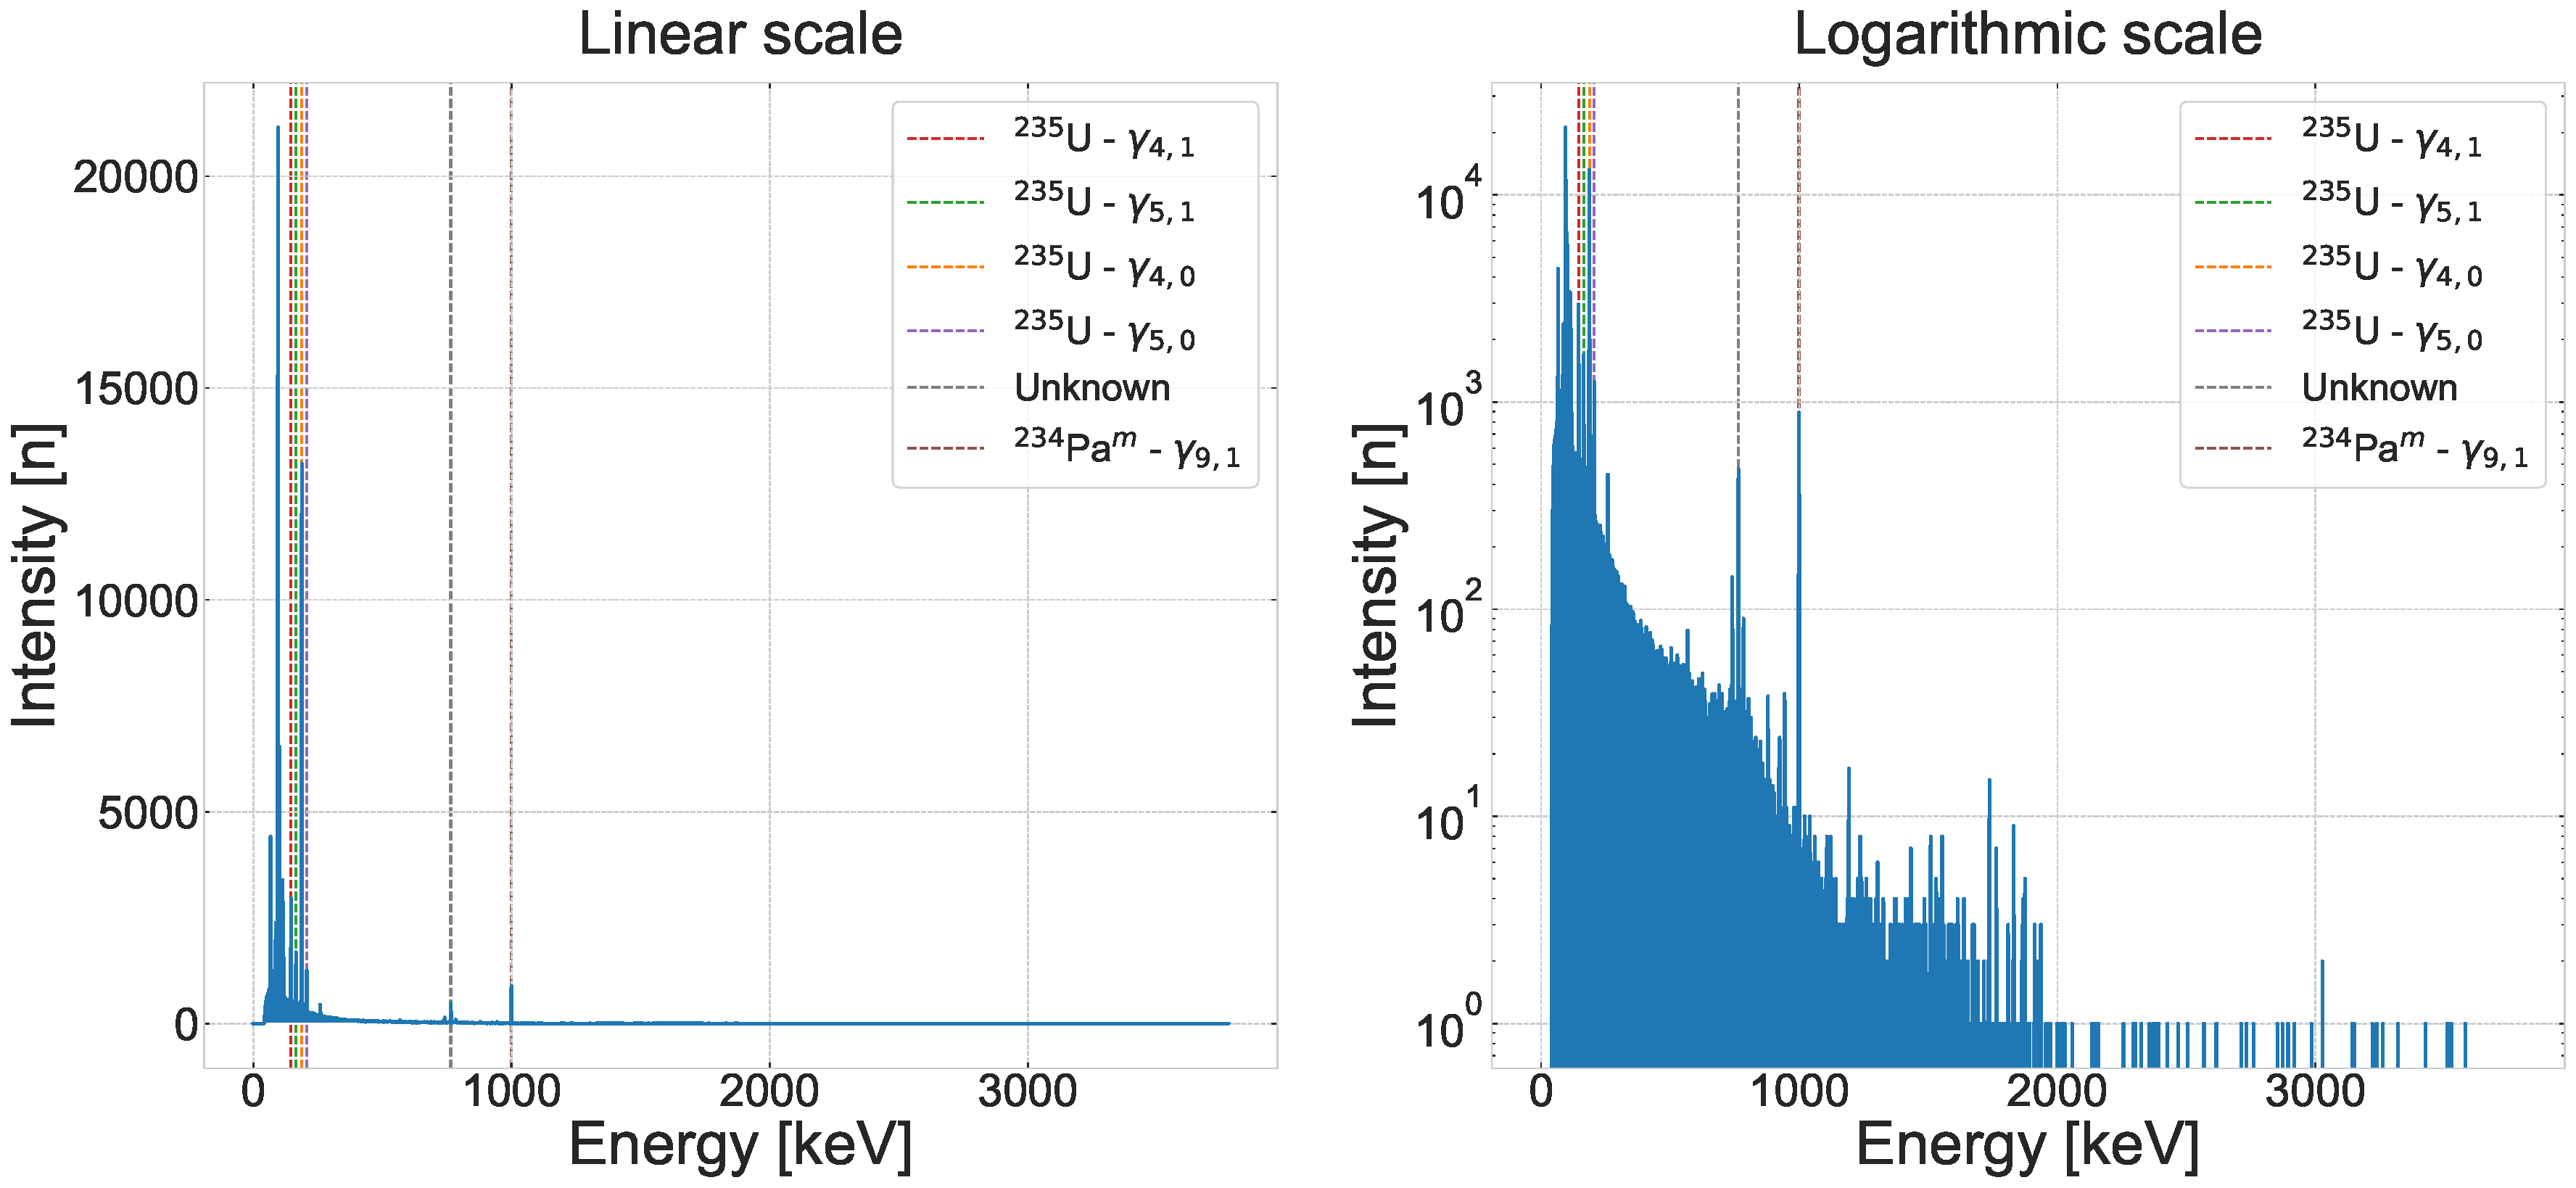
\includegraphics[width=\textwidth]{{images/full_spectra}.pdf}
    \captionof{figure}{Az általam vizsgált anyag teljes lemért gamma-spektruma. Az egyes karakterisztikus csúcsok színes, szaggatott vonallal vannak jelölve.} \label{fig:1}
\end{center}
\begin{center}
    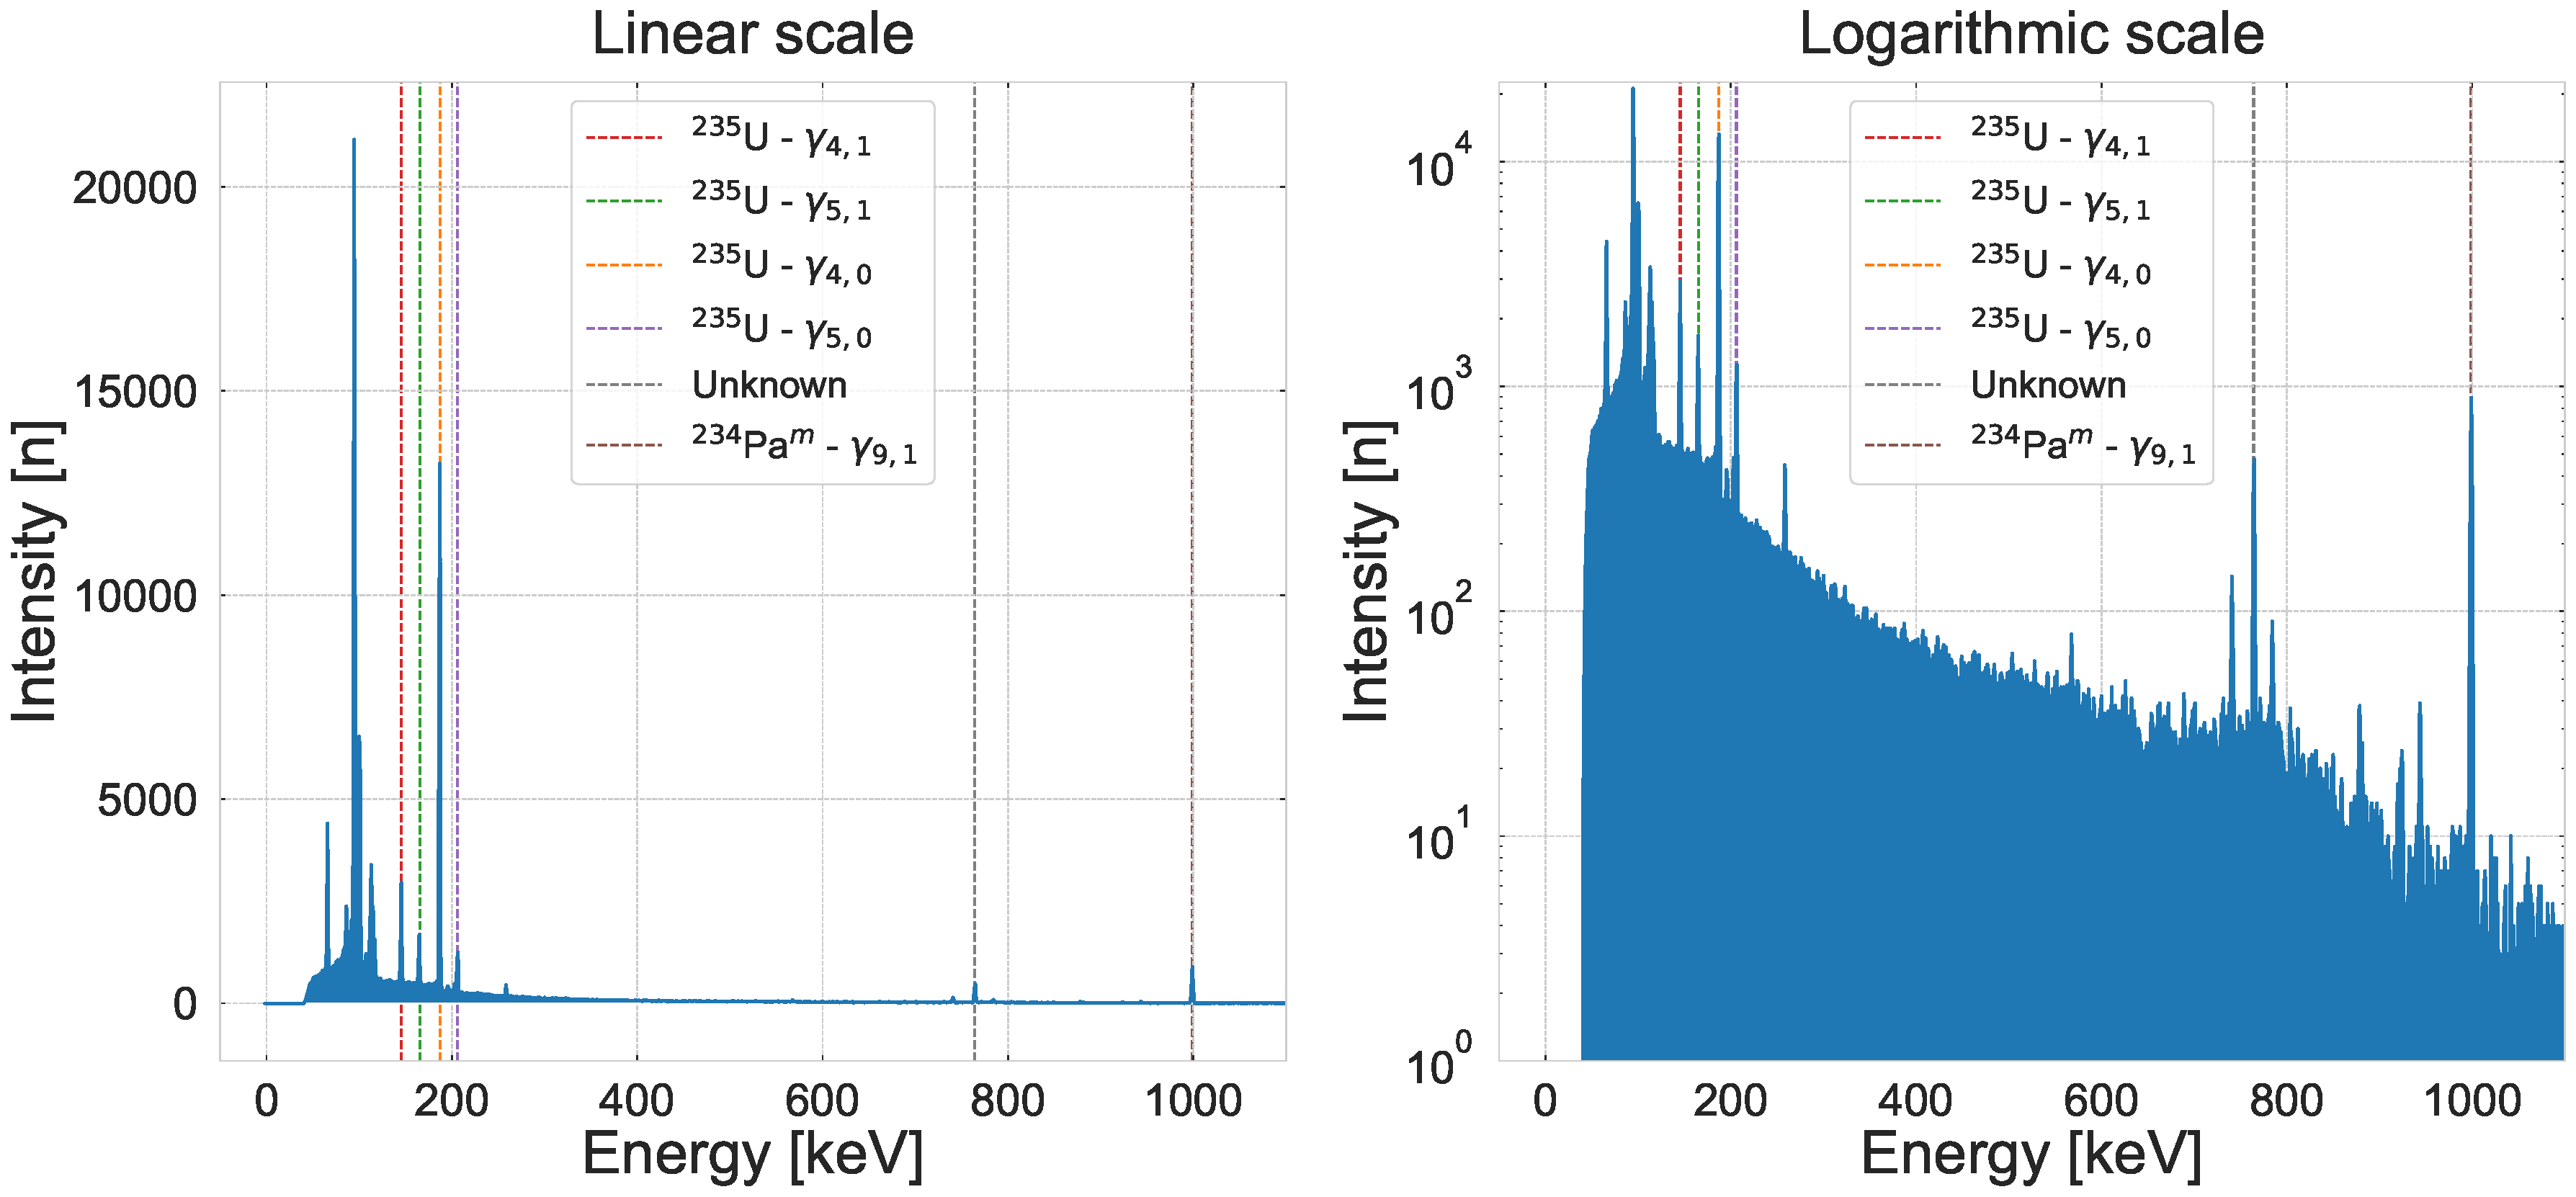
\includegraphics[width=\textwidth]{{images/spectra_lims_-50.00_1100.00_full_height}.pdf}
    \captionof{figure}{Az általam vizsgált anyag gamma-spektruma a $0\ \text{keV} - 1100\ \text{keV}$ intervallumban. Az egyes karakterisztikus csúcsok színes, szaggatott vonallal vannak jelölve.} \label{fig:2}
\end{center}
\begin{center}
    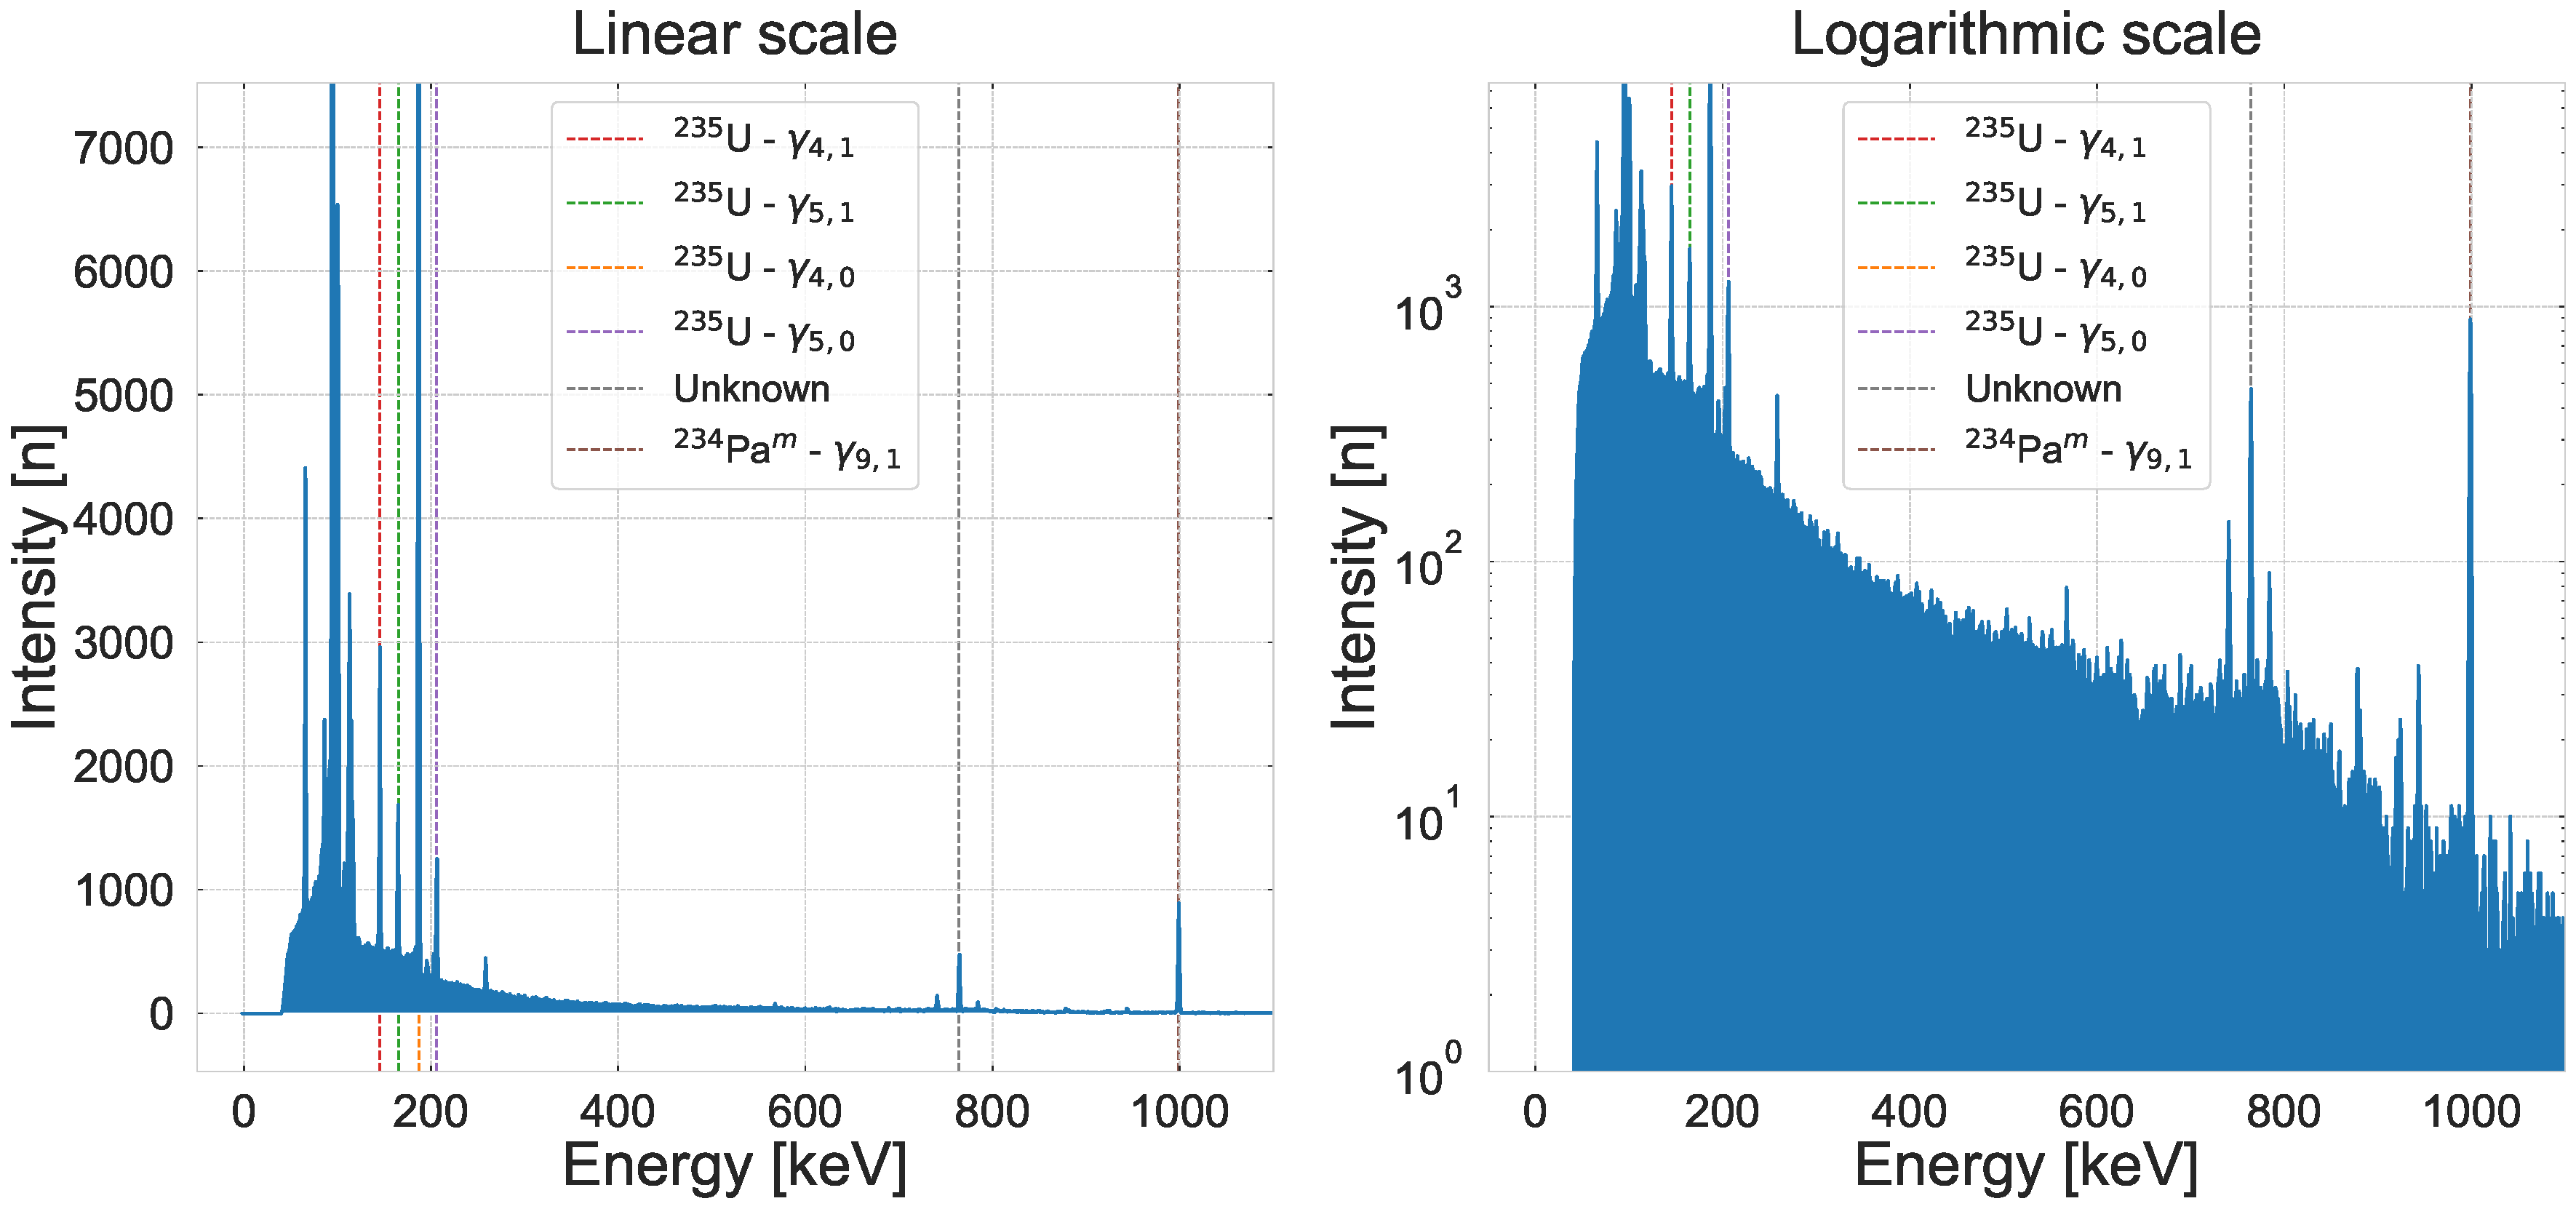
\includegraphics[width=\textwidth]{{images/spectra_lims_-50.00_1100.00_small_height}.pdf}
    \captionof{figure}{Az általam vizsgált anyag gamma-spektruma a $0\ \text{keV} - 1100\ \text{keV}$ intervallumban. Az ábrán a (\ref{fig:2})-es ábrán szereplő $y$-tengely alsó harmada van megjelenítve. Az egyes karakterisztikus csúcsok színes, szaggatott vonallal vannak jelölve.} \label{fig:3}
\end{center}
\vspace*{\fill}
\newpage
\topskip0pt
\vspace*{\fill}
\begin{center}
    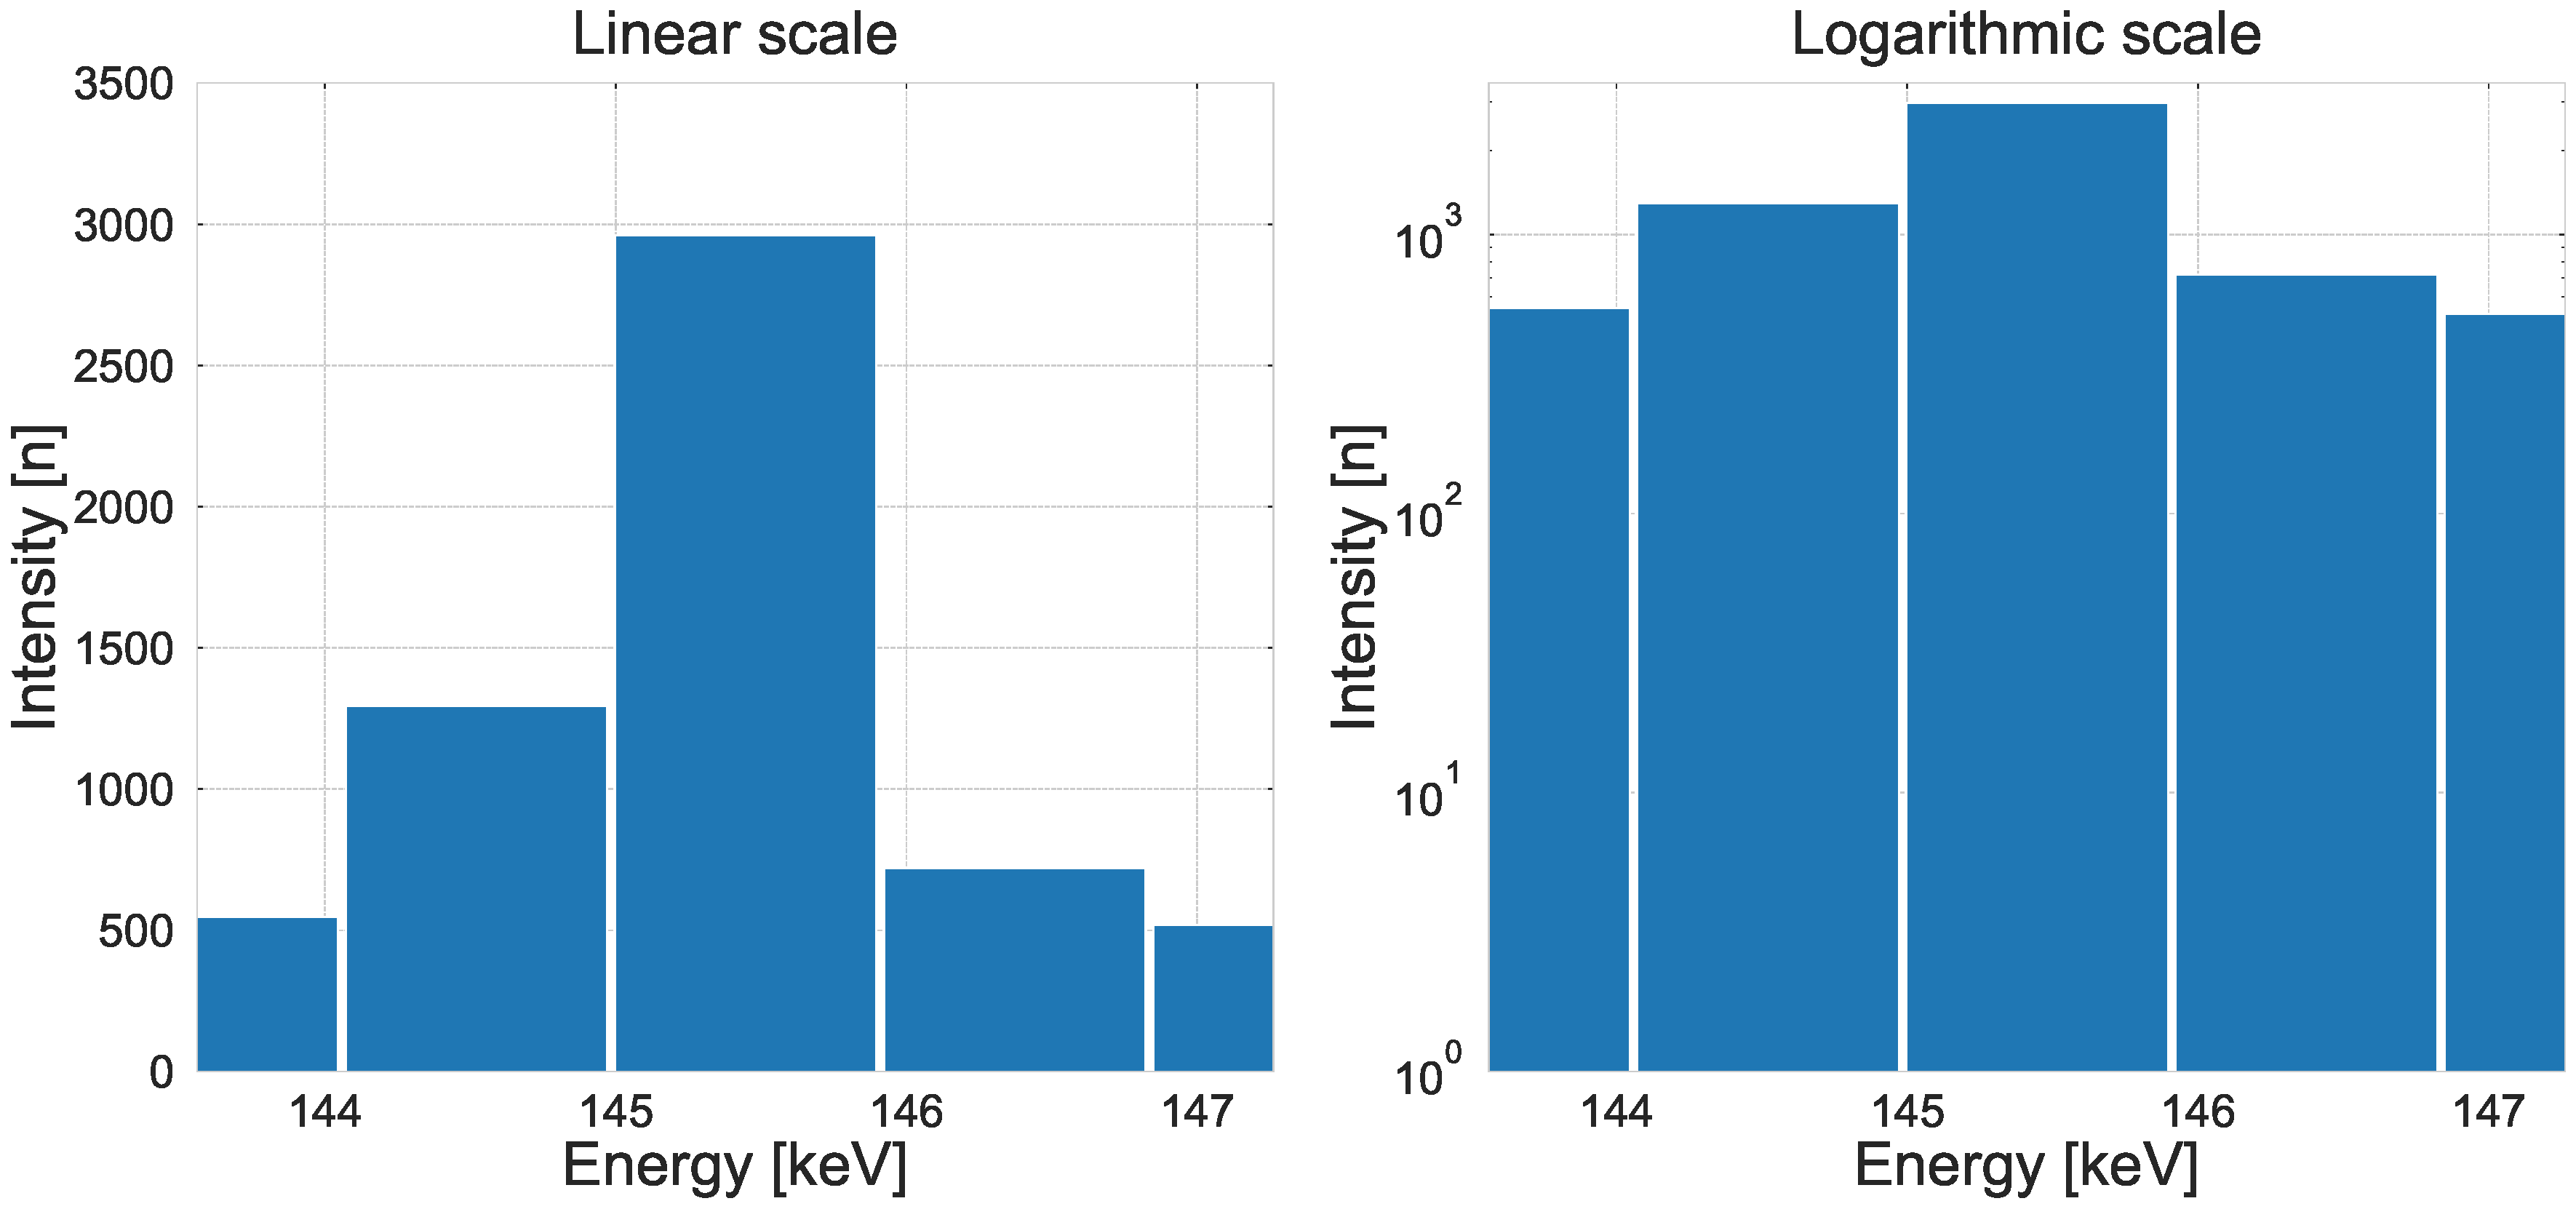
\includegraphics[width=\textwidth]{{images/spectra_lims_143.56_147.26_U235_g4_1}.pdf}
    \captionof{figure}{Az általam vizsgált anyag gamma-spektrumában található $^{235}$U, $\gamma_{4,1}$ tranziensből származó fotonjának foto-csúcsa.} \label{fig:4}
\end{center}
\begin{center}
    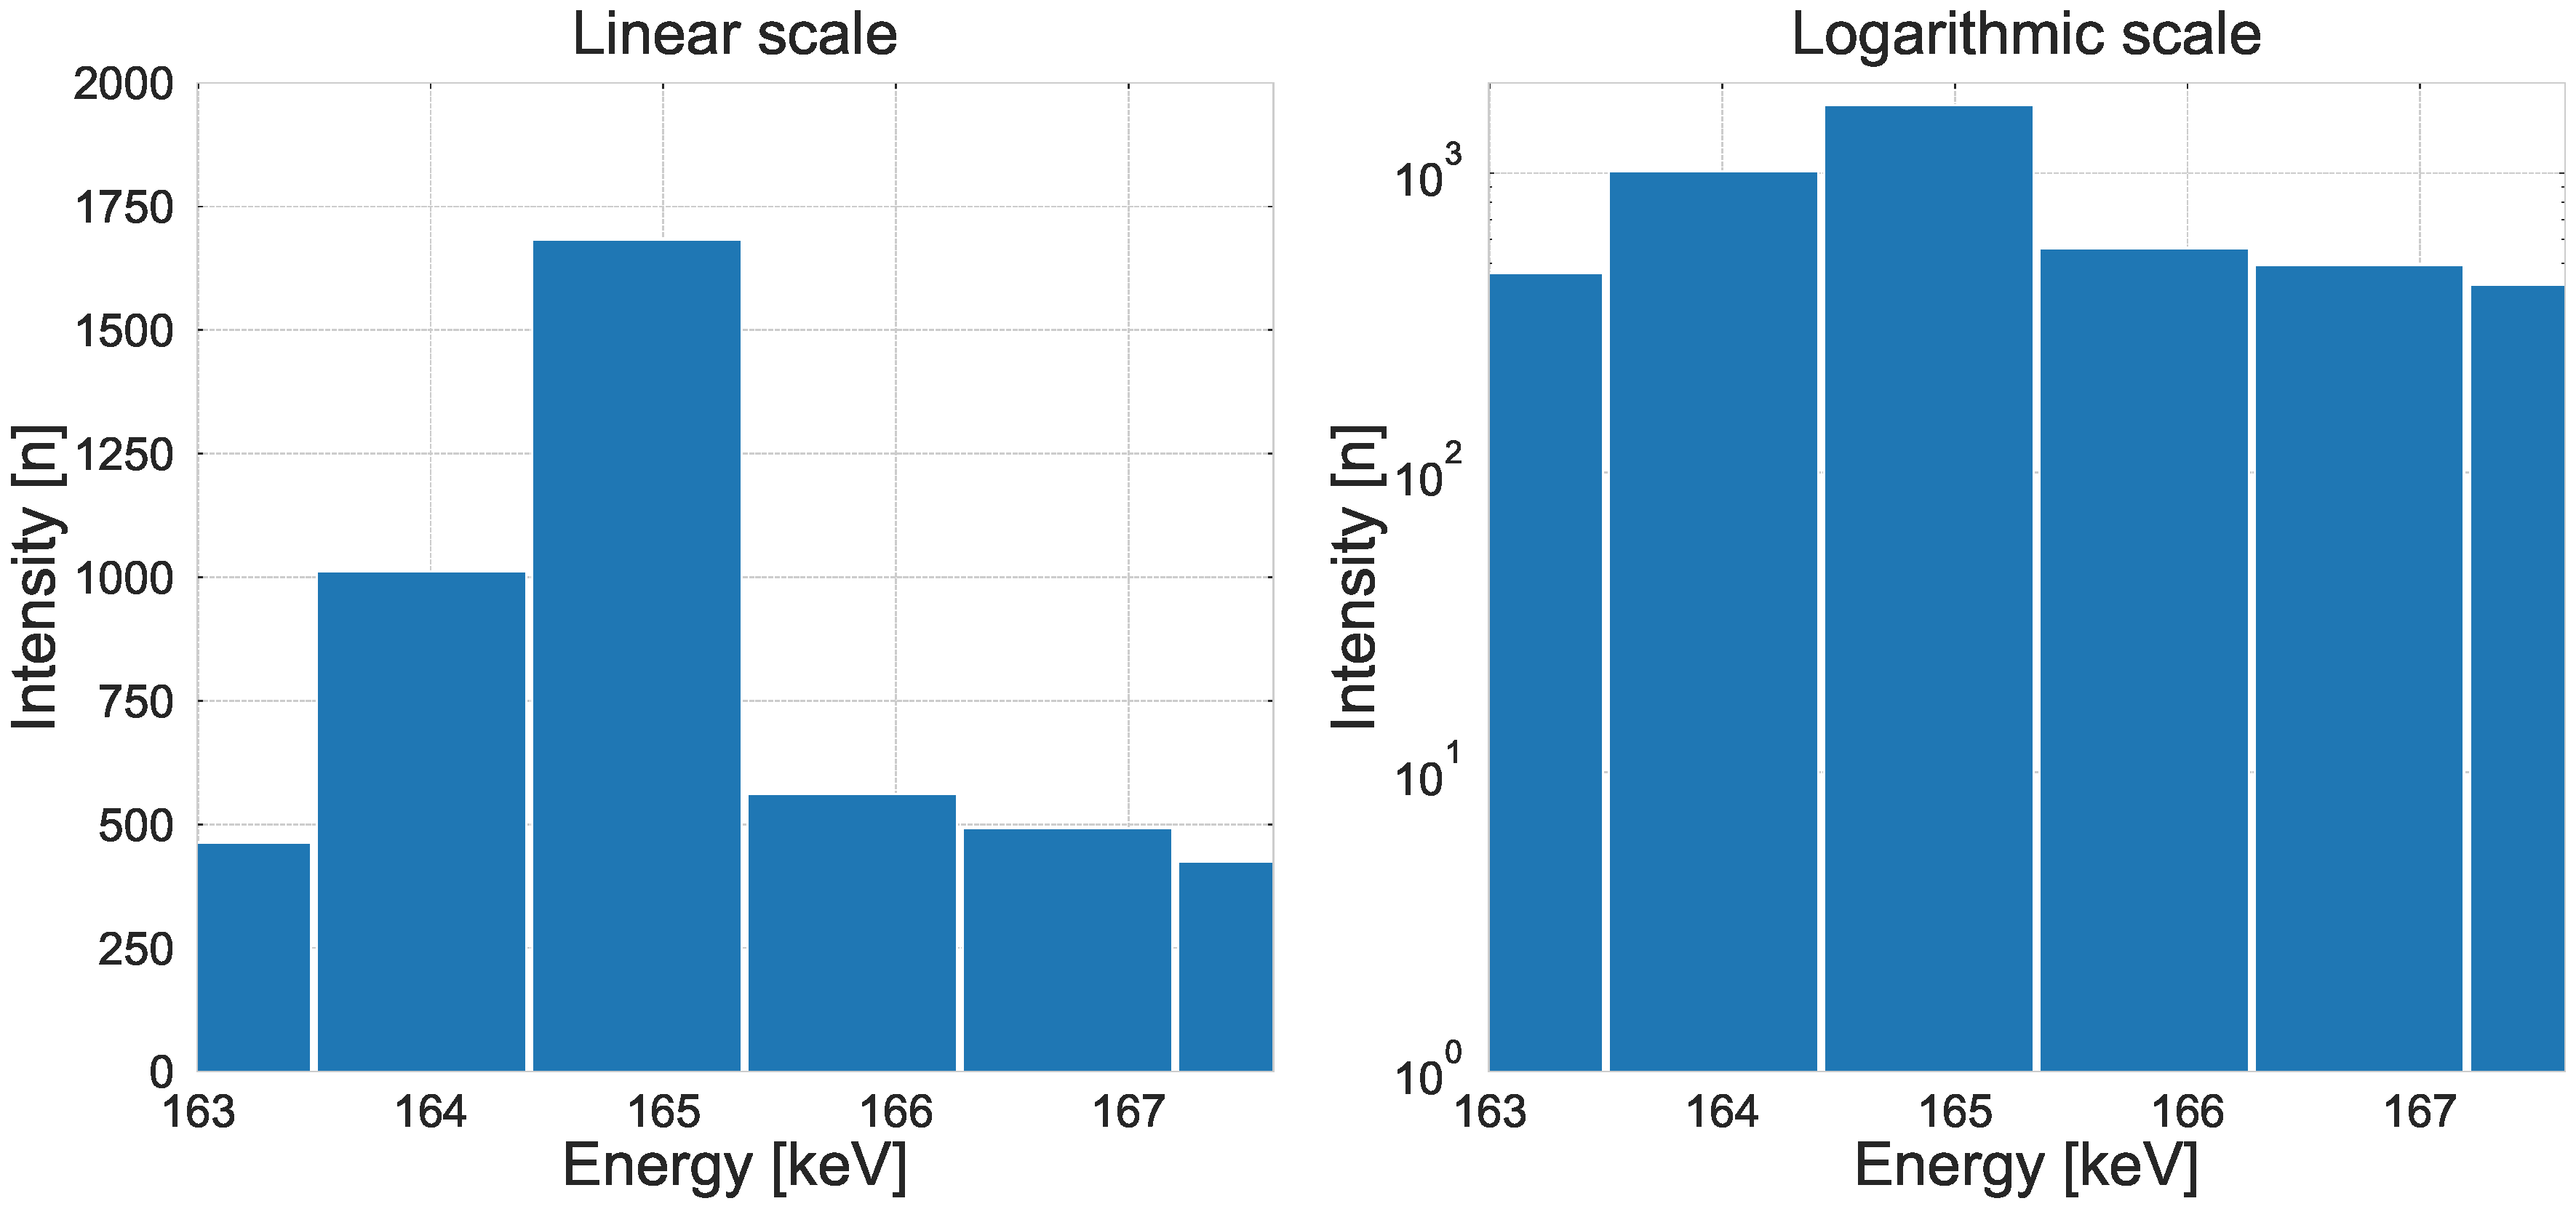
\includegraphics[width=\textwidth]{{images/spectra_lims_163.00_167.62_U235_g5_1}.pdf}
    \captionof{figure}{Az általam vizsgált anyag gamma-spektrumában található $^{235}$U, $\gamma_{5,1}$ tranziensből származó fotonjának foto-csúcsa.} \label{fig:5}
\end{center}
\begin{center}
    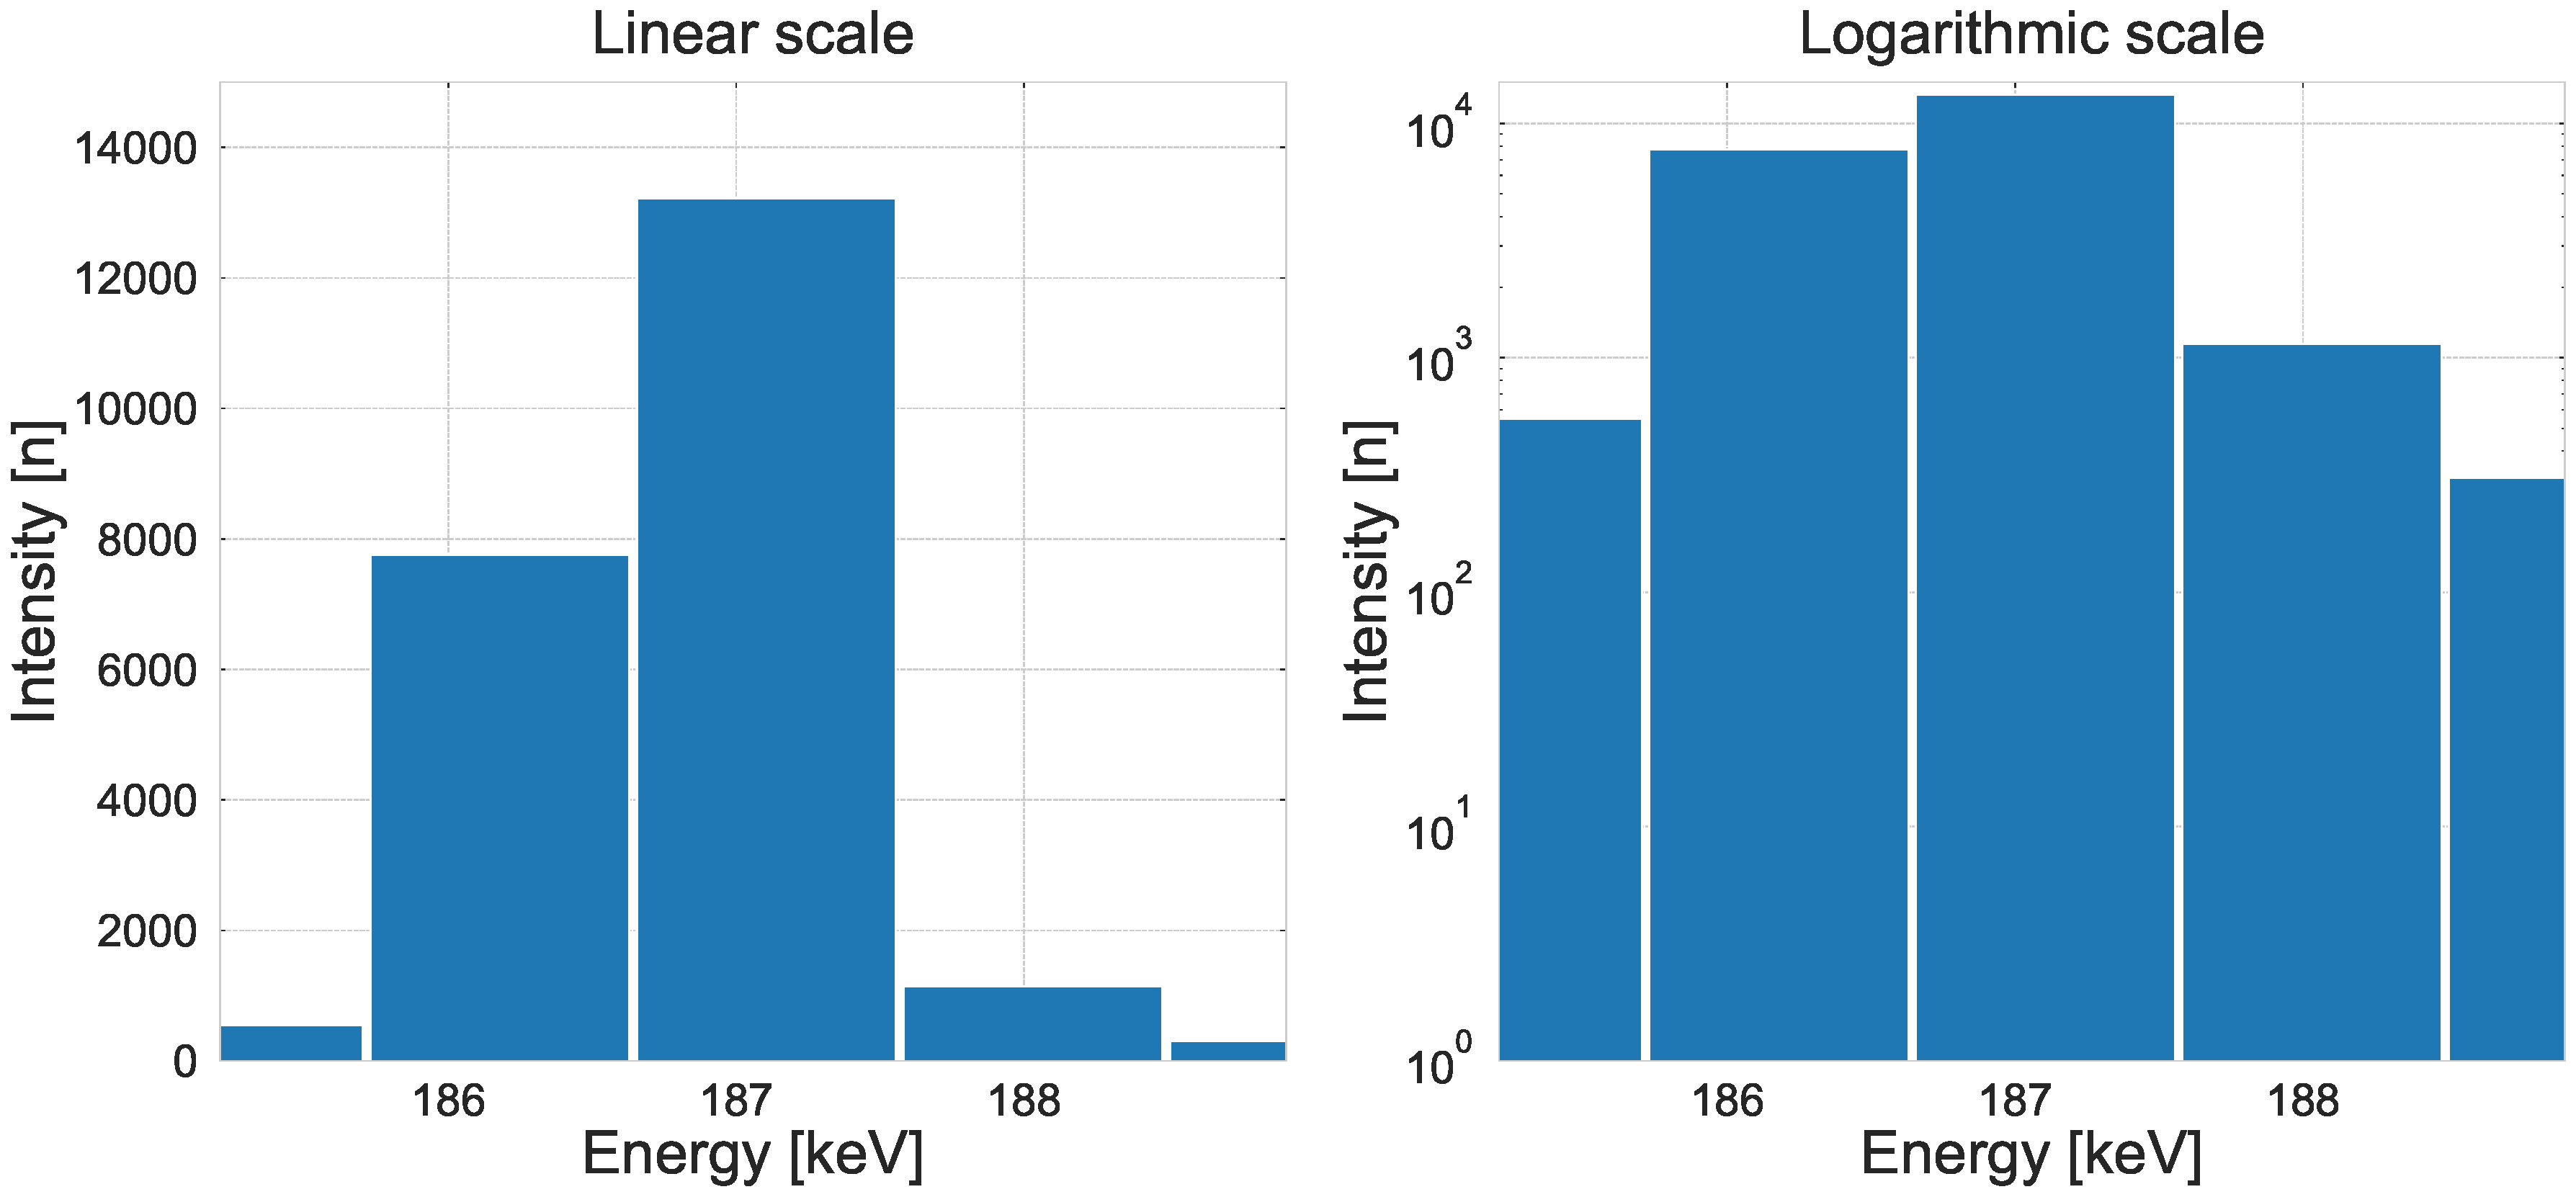
\includegraphics[width=\textwidth]{{images/spectra_lims_185.21_188.91_U235_g4_0}.pdf}
    \captionof{figure}{Az általam vizsgált anyag gamma-spektrumában található $^{235}$U, $\gamma_{4,0}$ tranziensből származó fotonjának foto-csúcsa.} \label{fig:6}
\end{center}
\vspace*{\fill}
\newpage
\topskip0pt
\vspace*{\fill}
\begin{center}
    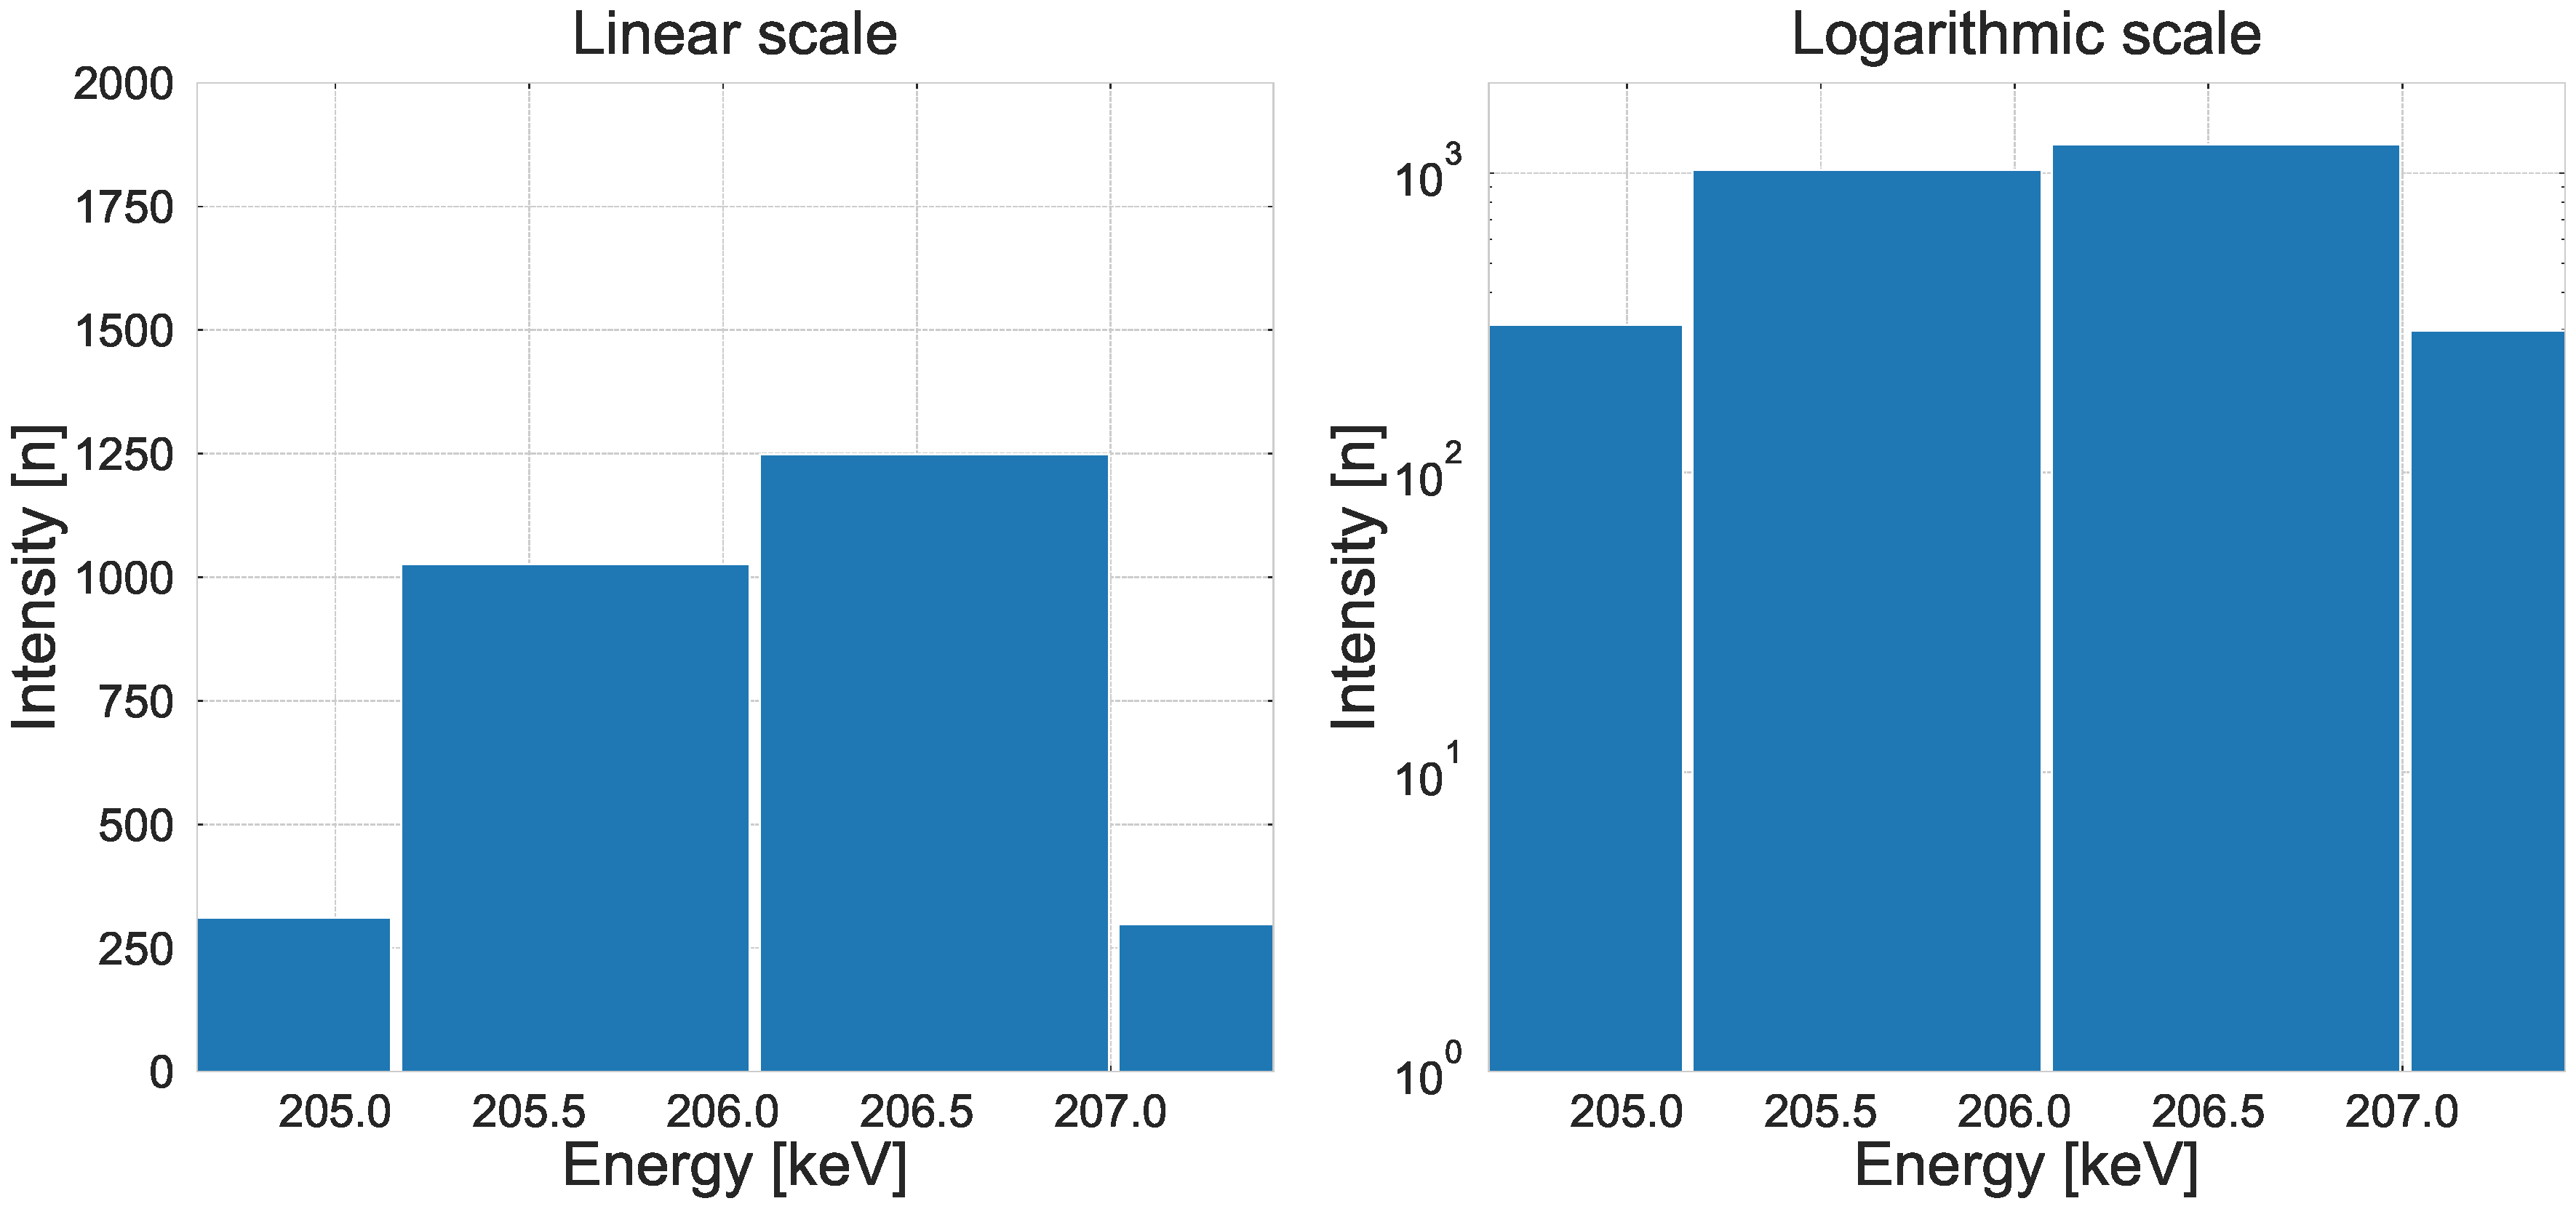
\includegraphics[width=\textwidth]{{images/spectra_lims_204.64_207.42_U235_g5_0}.pdf}
    \captionof{figure}{Az általam vizsgált anyag gamma-spektrumában található $^{235}$U, $\gamma_{6,0}$ tranziensből származó fotonjának foto-csúcsa.} \label{fig:7}
\end{center}
\begin{center}
    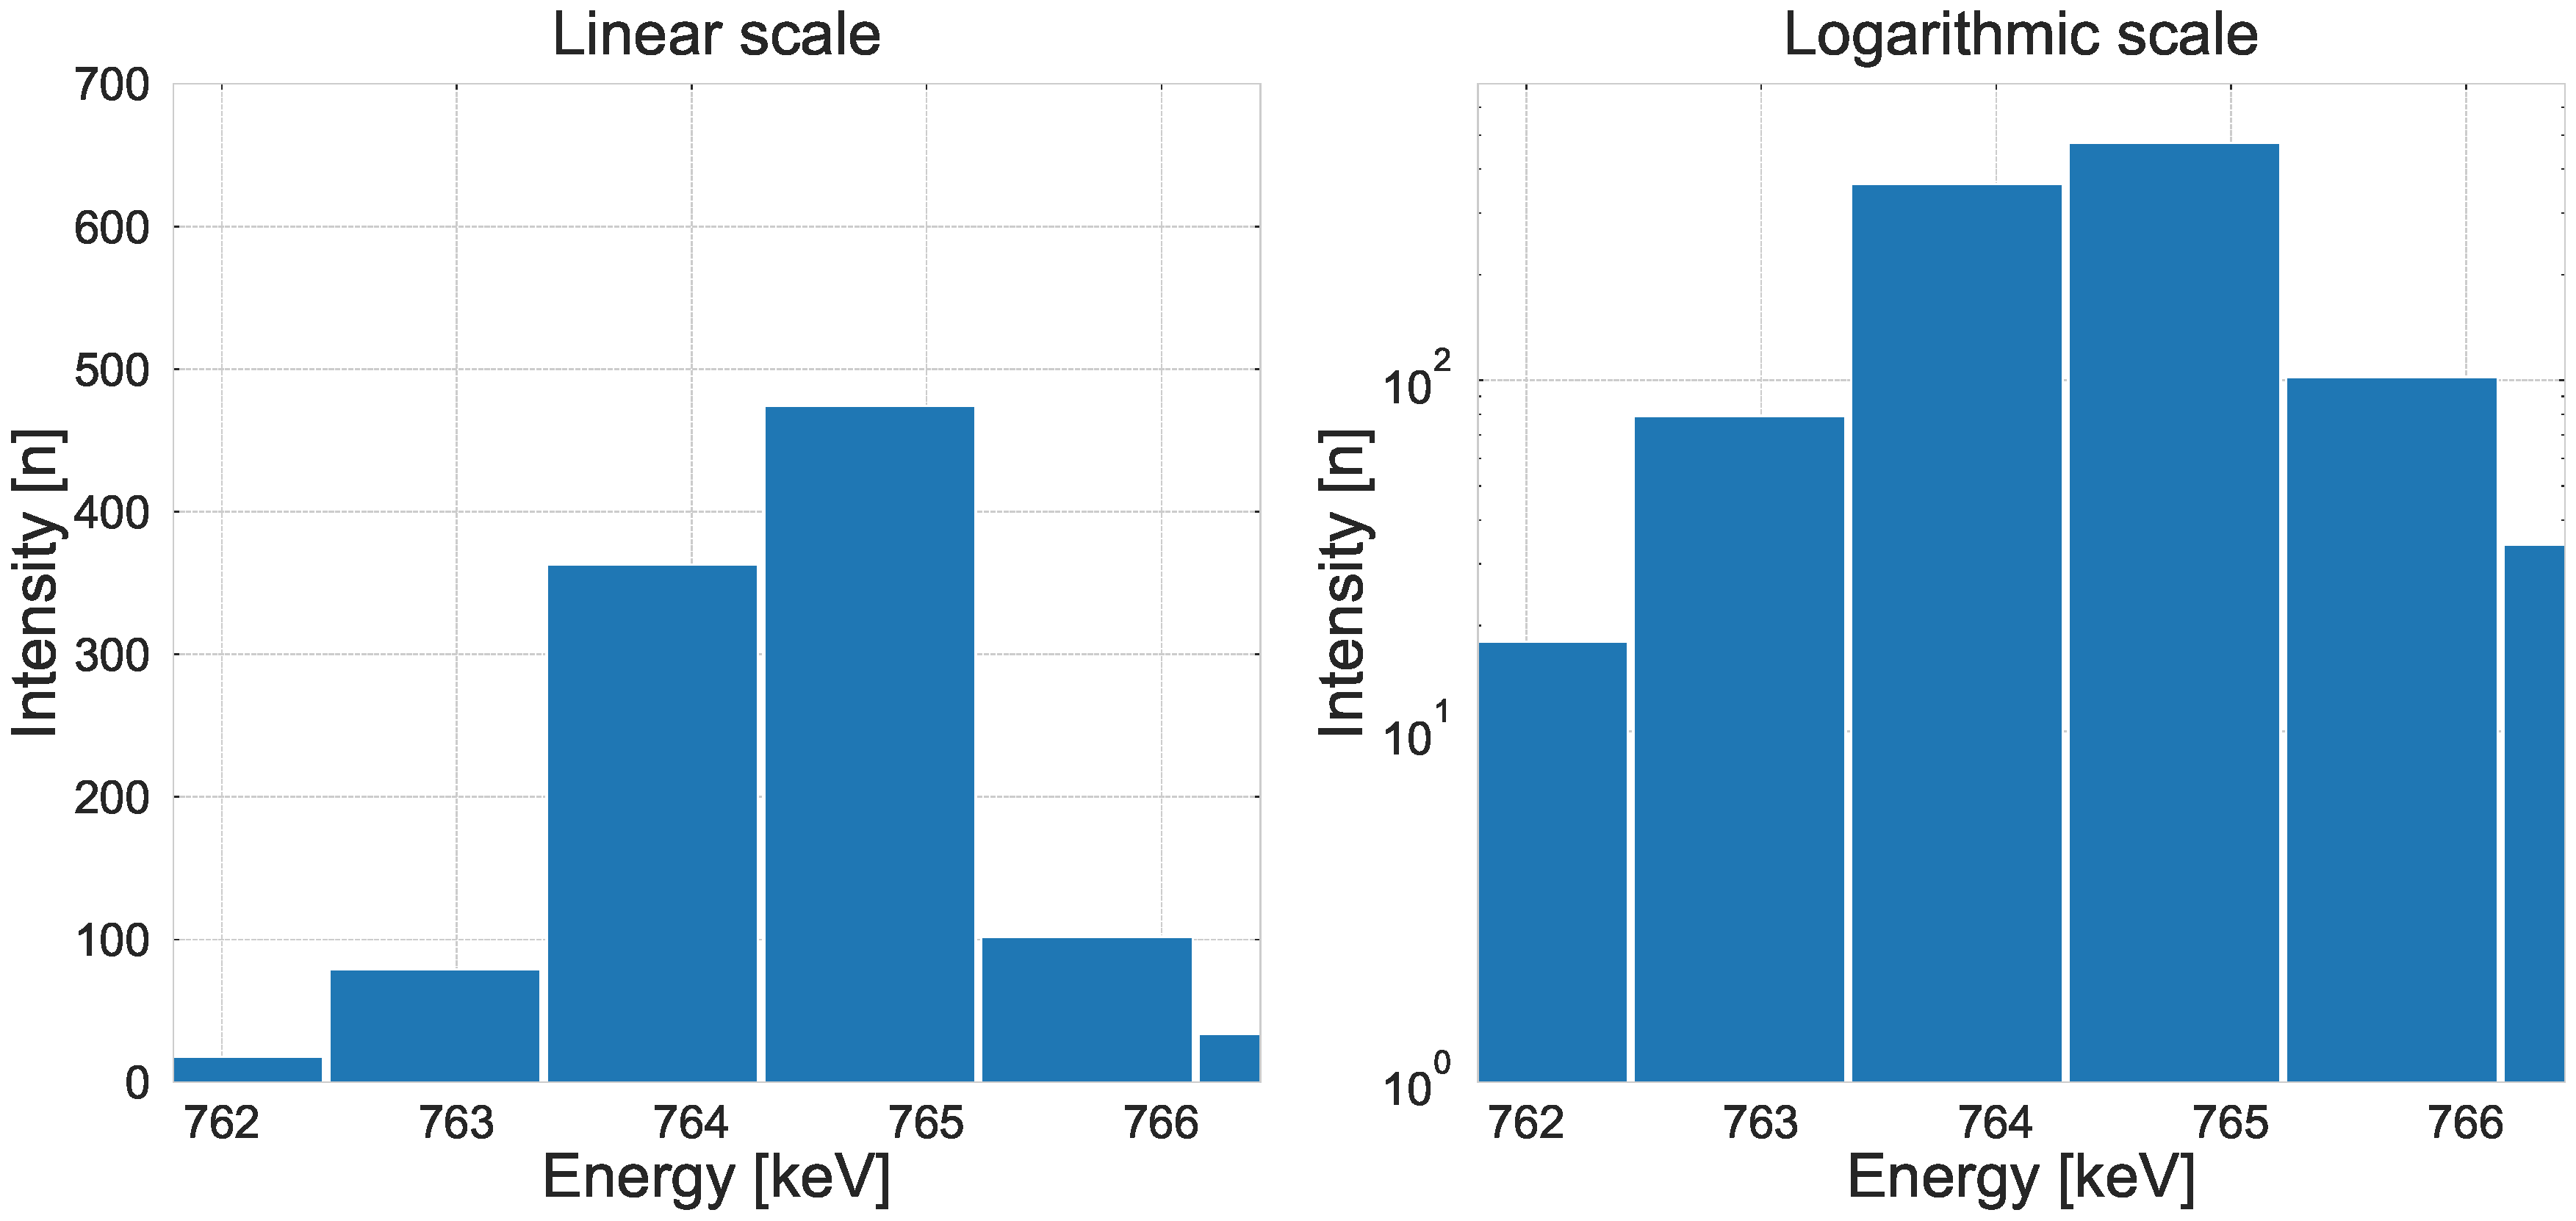
\includegraphics[width=\textwidth]{{images/spectra_lims_761.79_766.42_Unknown}.pdf}
    \captionof{figure}{Az általam vizsgált anyag gamma-spektrumában található $^{235}$U, $\gamma_{5,1}$ tranziensből származó fotonjának foto-csúcsa.} \label{fig:8}
\end{center}
\begin{center}
    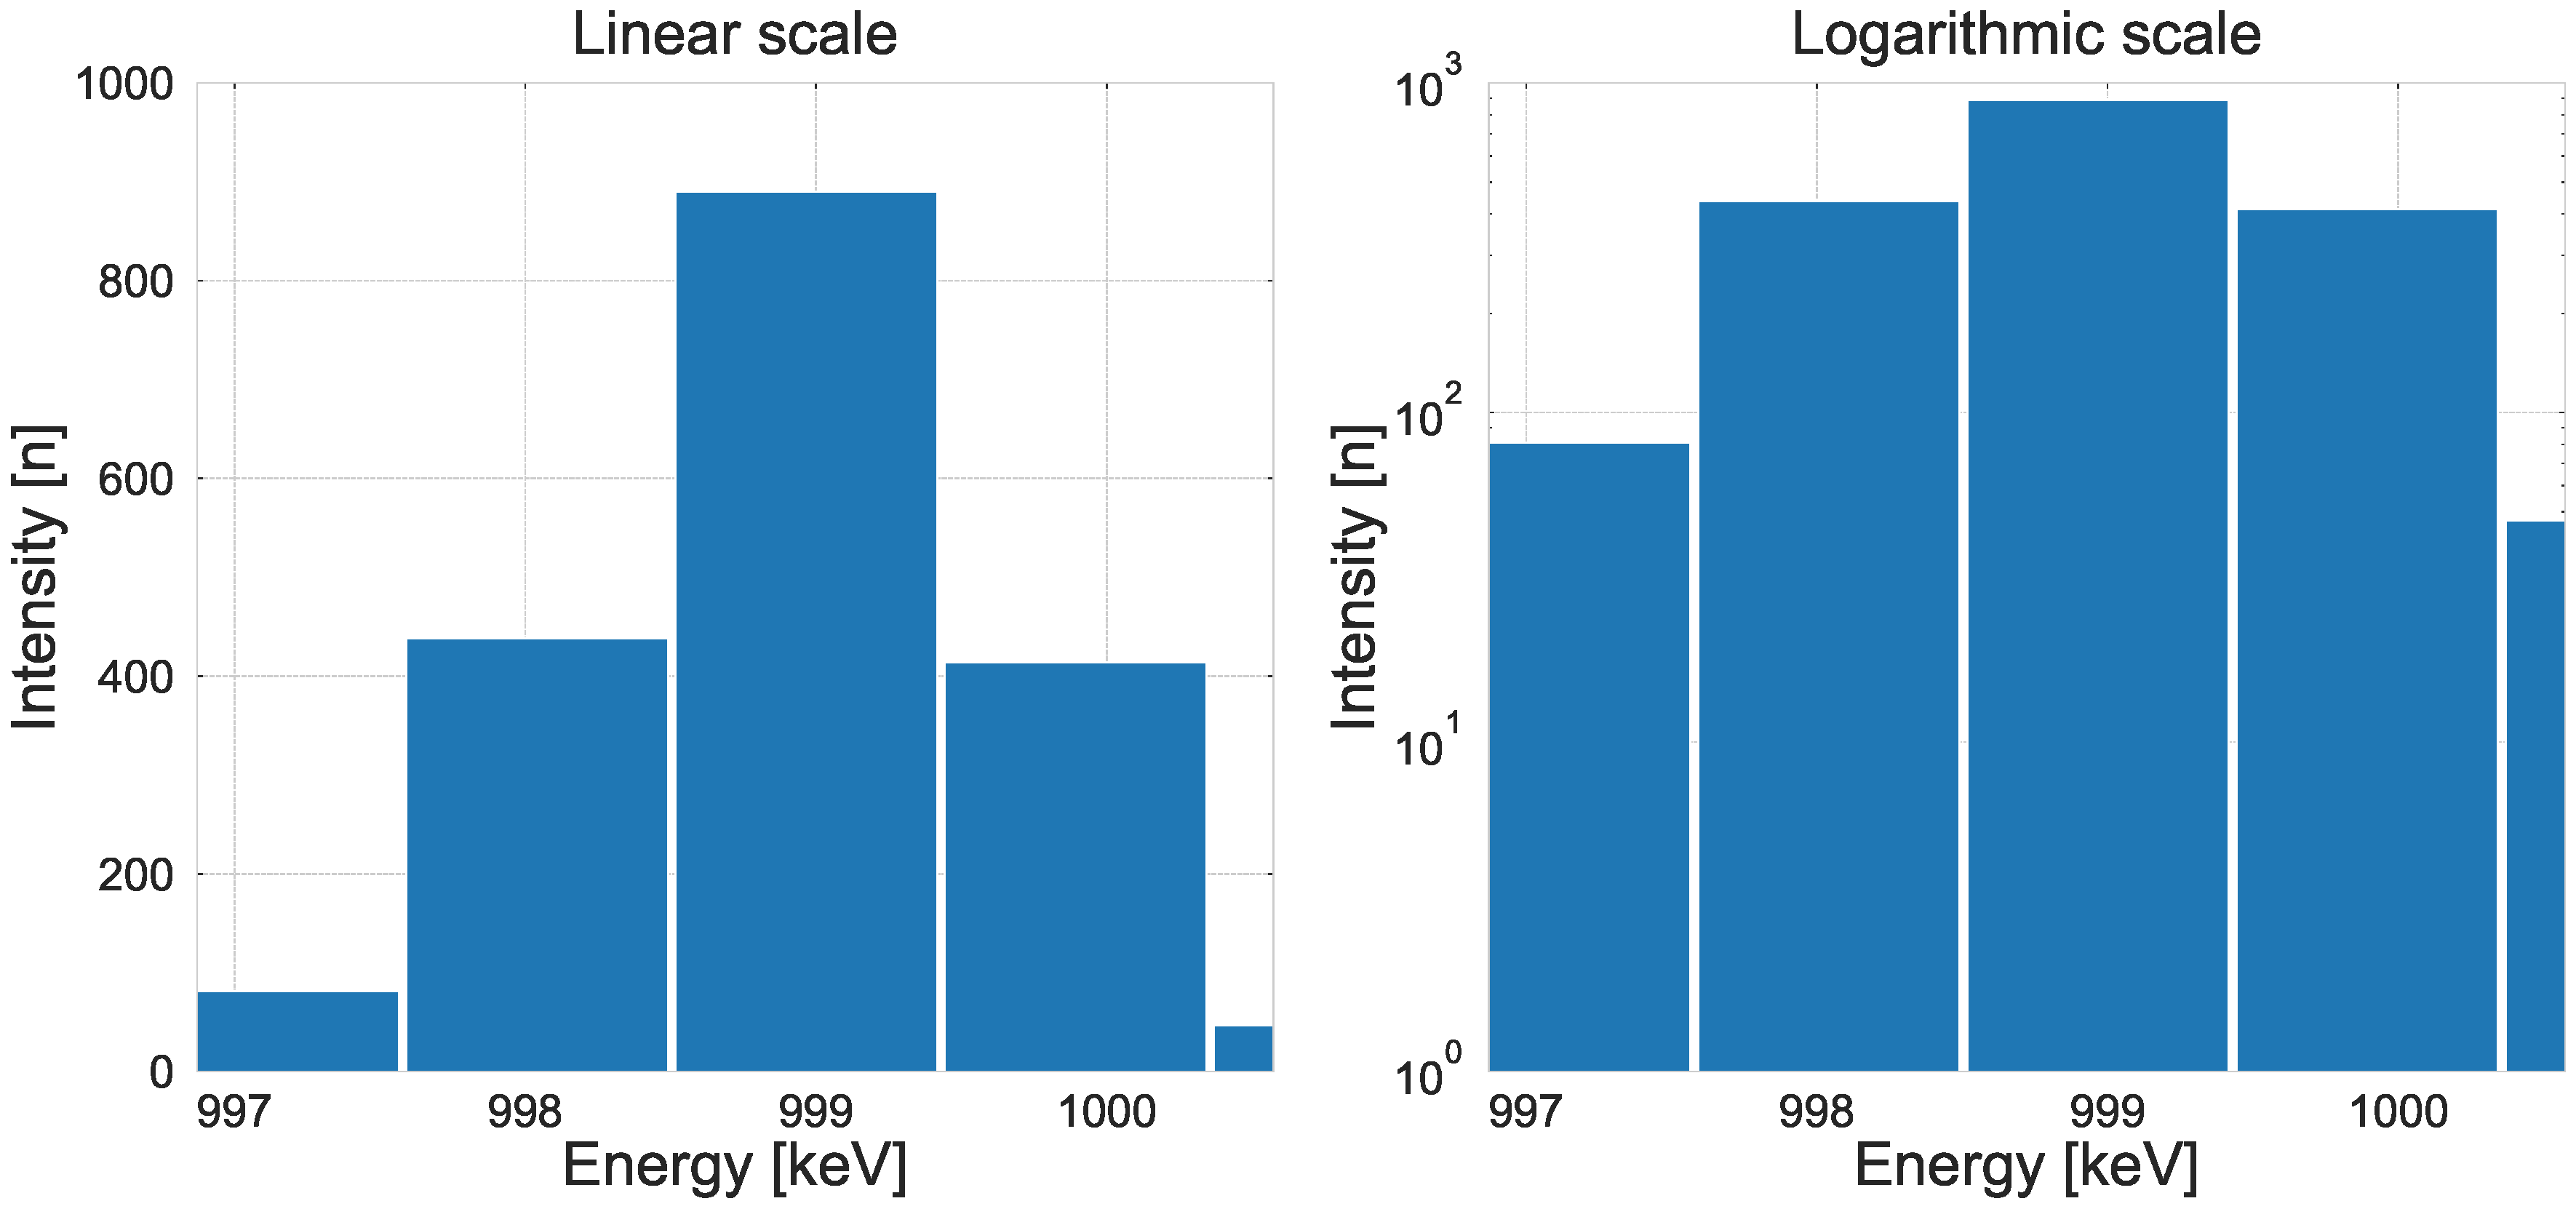
\includegraphics[width=\textwidth]{{images/spectra_lims_996.87_1000.57_Pam234_g9_1}.pdf}
    \captionof{figure}{Az általam vizsgált anyag gamma-spektrumában található $^{235}$U, $\gamma_{4,0}$ tranziensből származó fotonjának foto-csúcsa.} \label{fig:9}
\end{center}
\vspace*{\fill}